\chapter{Levantamento Bibliográfico}\label{cap:levbibliog}

Este capítulo apresenta uma breve introdução à \textit{Smart Cities}, \textit{Crowdsourcing}, contexto atual do desenvolvimento de programação voltada a aplicativos de transporte público e demais tópicos relativos ao desenvolvimento do trabalho.

\section{\textit{Smart Cities}}

O conceito de Cidades Inteligentes e o respectivo aumento no seu uso, pode ser reconhecido como o resultado do alto crescimento das tecnologias digitais na intenção de garantir um futuro sustentável. Embora o conceito seja empregado normalmente com o objetivo de elaborar estratégias que objetivem melhorar a qualidade de vida dos cidadãos, criando um futuro sustentável, o conceito por si só continua sendo usado em diferentes contextos e assim permanece um tanto ambíguo. Dessa forma faz-se necessário estabelecer um critério muito importante que o diferencia das cidades-conceito, o aspecto colaborativo entre os diversos interessados, mais comumente os cidadãos \cite{schuurman}. 

Um outro enfoque, mais empresarial, apresentado por \citeonline{walravens}, menciona que o conceito também pode ser empregado para caracterizar um grupo de organizações que intentam por revolucionar algum aspecto em uma região, entre os quais estão parques empresariais, o nível de escolaridade de uma população, o uso de tecnologias em contextos urbanos, o aumento da eficácia de governos e especialmente aquelas com foco em ICT. Walravens argumenta também que de maneira geral, o uso de serviços de telefonia móvel adquirem uma importância inevitável, já que é um sub aspecto de ICT e dessa forma grande importância na construção de uma Cidade Inteligente \cite{walravens}.

Em vista disso, sistemas operacionais desenvolvidos para \emph{smartphones} inspiram desenvolvedores a conceber aplicativos e serviços que aperfeiçoam a vida nas cidades de diversas formas diferentes, como por exemplo, facilitando acesso à informação sobre o transporte publico. Além disto, à medida que os \emph{smartphones} se tornam mais acessíveis e populares, cria-se o desejo de que se tornem eminentes ferramentas na busca de uma cidade mais inteligente \cite{walravens}.

\section{\textit{Crowdsourcing}}

Outro aspecto importante  a ser mencionado é a caracterização de \emph{crowdsourcing}, no que tange inteligência coletiva. À grosso modo, entende-se inteligência coletiva como quando indivíduos de um determinado grupo, que possui interesse por determinado assunto, combinam seus conhecimentos a fim de encontrar a solução para um determinado problema.  Através da interação social, o conhecimento individual é compartilhado, corrigido, processado, enriquecido e avaliado. Normalmente, os resultados colhidos são melhores que os obtidos por um único indivíduo. Talvez a aplicação mais difundida desse conceito seja a Wikipedia  \cite{schuurman}. 

Por conseguinte, a ponte que se estabelece entre \emph{crowdsourcing} e \emph{smart cities} acompanha o advento dos \textit{smartphones}. Para \citeonline{kanhere}, as melhorias no poder de processamento, sensoriamento e capacidades de armazenamento permite que telefones celulares sejam comparados a dispositivos de computação. Esse fenômeno abre margem ao surgimento de um novo paradigma, denominado pela literatura de sensoriamento participativo, cuja ideia principal gira em torno de capacitar um cidadão comum a coletar e compartilhar dados de sensoriamento do ambiente em que está inserido, a partir de seu telefone celular \cite{kanhere}.

Ainda segundo Kanhere, sensoriamento participativo possui quatro vantagens principais sobre redes de sensores tradicionais (já que esta necessita de uma gama considerável de dispositivos sem fio, principalmente em áreas urbanizadas), sendo elas: custo de implementação baixo, já que usa telefones celulares e Wi-Fi; uma ampla mobilidade e cobertura proporcionada pelas operadoras de telefonia; economias de escala proporcionadas pelo uso de celulares; a facilidade assegurada pelas lojas de aplicativos e também as inúmeras formas de desenvolvimento de software disponíveis para sistemas operacionais de dispositivos móveis \cite{kanhere}. 

\section{Arquiteturas de rede}

A proposta de uma arquitetura para \sigla{DTN}{\emph{Delay Tolerant Networks}} (\emph{Delay Tolerant Networks}) surgiu a partir da necessidade de que dispositivos capacitados para operar nas redes móveis e sem fio (smartphones e tablets, por exemplo) operem em qualquer lugar e instante de tempo, mesmo na ausência de uma infra-estrutura de rede. Assim, alguns problemas como conectividade não contínua e atrasos muito longos, podem ser solucionados  \cite{vendramin2012c}.

%http://ipnsig.org/wp-content/uploads/2012/07/DTN_Tutorial_v2.05.pdf - warthman
Segundo \citeonline{warthman}, DTNs foram projetadas originalmente para uso interplanetário, onde a tolerância a atrasos é de extrema importância. No entanto, muitas aplicações terrestres podem ser vislumbradas com o uso de DTNs, especialmente quando trata-se de tecnologias sem fio (\textit{wireless}), tais como RF.

Entretanto, o modelo atual no qual funciona a Internet, largamente apoiada no protocolo TCP/IP, vai de encontro com alguns princípios de uma arquitetura DTN. A comunicação utilizando TCP/IP no que se refere à conectividade intermitente, na qual não há um caminho entre um nó origem e um nó destino na rede, por exemplo, não funciona \cite{warthman}. Ainda, segundo \citeonline{warthman}, os protocolos de Internet atuais não suportam longos períodos de espera por uma resposta (um \sigla{ACK}{\textit{Acknowledge}}, \textit{Acknowledge}).

A arquitetura DTN se apoia num método muito antigo chamado \emph{store-carry-forward} (armazenar, transportar e encaminhar), onde informações (ou fragmentos dela) são armazenados em um local de armazenamento em um nó e movidos para outro nó através de um caminho que eventualmente atinja o destino \cite{warthman}. \citeonline{warthman} enumera as razões na qual o armazenamento persistente em uma DTN é necessário, que são a possibilidade de que a comunicação entre os nós não esteja indisponível por um longo tempo, a disparidade na velocidade de transmissão e recepção de informações entre os nós e a transmissão (retransmissão) de informações em caso de erros ou de não aceitação de recebimento por um determinado nó.

No que tange arquiteturas de rede, há também a arquitetura \sigla{P2P}{\emph{Peer-to-Peer}} (\emph{Peer-to-Peer}) capaz de fornecer recursos de rede com sobreposição e auto-organização distribuída, com o intuito de prover uma distribuição eficiente dos dados. O mecanismo básico de funcionamento consiste em pares, nos quais uma entidade presta e, ao mesmo tempo, consome os recursos oferecidos por outras entidades que compõe o sistema. Outras características que estes sistemas apresentam, normalmente, são auto-organização, tolerância a falhas e escalabilidade \cite{italianos}.

Com base em todos esses conceitos, estabelece-se, a seguir, um breve estado da arte registrado na literatura, no que se refere à área de desenvolvimento de aplicativos para plataformas móveis dentro da ideia de \emph{crowdsourcing} e \emph{smart cities}.

\section{Estado da Arte}

Conforme já relacionado na Introdução, \citeonline{sujatha} propuseram um sistema chamado MBTS para que qualquer pessoa obtenha informações de um determinado ônibus através de um aplicativo móvel. 

Três são os atores do sistema: os passageiros, os chamados ``coordenadores'' do ônibus e as pessoas que estão aguardando em um ponto. Todos os atores necessitam de um \textit{smartphone} com sistema operacional Android conectado à Internet. Continuamente, os passageiros e os ``coordenadores'' alimentam um banco de dados com informações sobre o ônibus. Essas informações podem ser as coordenadas do ônibus, obtidas através do GPS integrado ao \emph{smartphone}, ou até mesmo a ``situação'' do ônibus -- se ele está lotado ou vazio, se houve algum acidente, se o ônibus está atrasado, entre outros. Essas informações ficam armazenadas em um banco de dados para serem acessadas, posteriormente, por alguém que esteja utilizando o aplicativo, principalmente usuários que estão aguardando um ônibus em algum ponto. 

A arquitetura do MBTS pode ser observada na Figura \ref{fig:archMBTS}. Basicamente, consiste de duas aplicações, uma Web e outra Android. A primeira permite o registro de usuários e ônibus e a segunda é utilizada para rastreio. A aplicação Web, desenvolvida em \sigla{JSP}{\textit{JavaServer Pages}} (\textit{JavaServer Pages}), é voltada para o administrador do sistema e também funciona como um \textit{``middleware''} para que a aplicação Android se conecte ao banco de dados e armazene informações \cite{sujatha}.

Uma outra pesquisa neste área de acompanhamento de ônibus, envolve a utilização de \sigla{RF}{Radio Frequência} (Radio frequência). Foi desenvolvida por \citeonline{paradells}.

Os autores propõe a utilização de uma rede de dados composta por transmissores e receptores RF. Os transmissores situam-se nos ônibus, os quais transmitem informações para os receptores, que situam-se nos pontos de ônibus que, basicamente, são os nós da rede. Assim que um ônibus se aproxima de um ponto de ônibus - nó - inicia a transmissão de informações relevantes, captadas por sensores atrelados ao veículo. Essas informações podem ser usadas/acessadas por um usuário que está aguardando no referido ponto de ônibus. 

\begin{figure}[h]
\begin{center}
    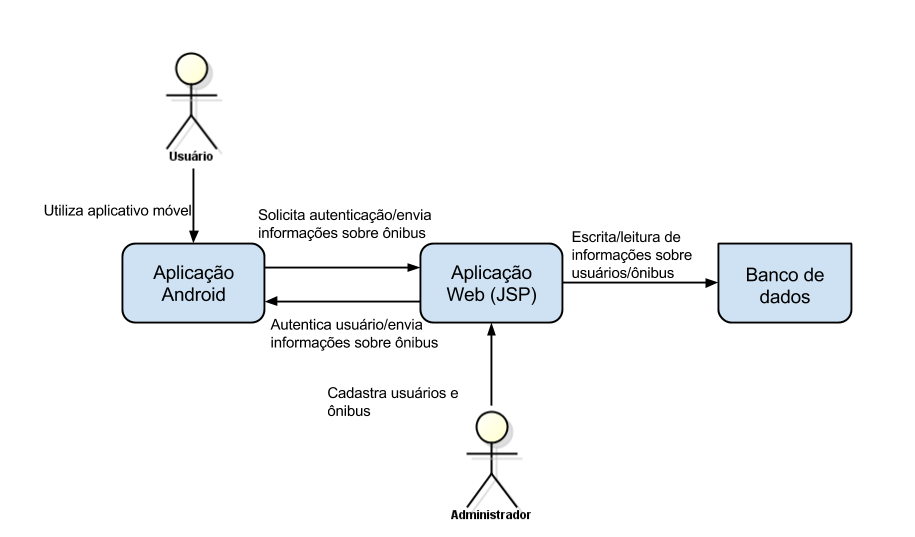
\includegraphics[width=1\columnwidth]{../figs/arquitetura_mbts.png}
    \caption{Arquitetura do MBTS.}Fonte: Adaptado de \citeonline{sujatha}.
    \label{fig:archMBTS}
\end{center}
\end{figure}

Uma limitação do sistema baseado em RF, e percebida pelos próprios autores, diz respeito à distância entre o ônibus e os nós da rede (neste caso os pontos de ônibus). Uma vez que sensores baseados em radio frequência possuem limitações de distância e na transmissão dos dados, acabam limitando a velocidade desenvolvida pelo veículo, o que torna o projeto inviável. 

Ainda, as informações só podem ser coletadas por usuários que já estão próximos ao veículo (ou em pontos de ônibus próximos ao veículo). Isso acaba tirando o propósito de acompanhamento ou rastreio de ônibus, pois o mesmo já está próximo do ponto, e pode ser visualizado por um usuário sem o auxílio de um sistema específico para tal.

\citeonline{alves} apresentaram um sistema -- chamado de \emph{Trip-planner} -- para planejar rotas em tempo real, para pessoas que utilizam transporte público em Lisboa. O sistema consegue informar quais são as melhores rotas e o tempo estimado de viagem para um determinado destino, baseados na estimativa de quantos veículos estão trafegando e quais são suas velocidades.

Informações de tempo-real são coletadas através do GPS equipado nos ônibus. Essas informações são utilizadas em um servidor (o que os autores chamam de \emph{Data Center}) para atualizar históricos e melhorar as estimativas, uma vez que é utilizado um algoritmo para predição de tempos de viagem. Esses históricos se referem à relatórios de quatro meses, com informações sobre tempos de viagem e velocidades dos veículos. Essas informações são analisadas e passam por um classificador, e uma vez processadas, são repassadas para qualquer dispositivo móvel conectados em uma rede sem fio, através de \emph{broadcast} \cite{alves}.

A Figura \ref{fig:archLisbon} descreve de forma simplificada o sistema proposto por \citeonline{alves}. Nota-se claramente que dados históricos e de tempo-real são coletados com o auxílio do GPS instalado no ônibus. Esses dados passam pelo \emph{Data Center} e são utilizados como entrada para um algoritmo de predição. Uma vez processados, distribuem-se os dados para dispositivos móveis através de \emph{broadcast.}

\begin{figure}[h]
\begin{center}
    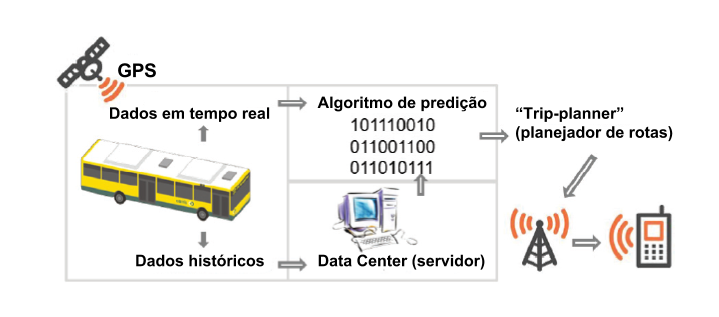
\includegraphics[width=0.85\columnwidth]{../figs/arquitetura_tripplanner.png}
    \caption{Arquitetura do \emph{Trip-planner}.}Fonte: Adaptado de \citeonline{alves}.
    \label{fig:archLisbon}
\end{center}
\end{figure}

\section{Discussões}
% inserir motivação
Conforme já discutido na Introdução, a principal motivação para o desenvolvimento deste projeto é implementar um aplicativo de acompanhamento de ônibus para dispositivos móveis - \textit{smartphones} - que utilize uma rede descentralizada. 

Espera-se que o aplicativo a ser desenvolvido seja de grande ajuda ao dia a dia dos passageiros do transporte coletivo e que, de alguma, forma traga informações de qualidade aos usuários, bem como lhes ofereça uma maior economia de tempo e torne o processo de decisão, sob qual ônibus tomar ou qual rota seguir, descomplicado.

Em termos de arquiteturas de rede, decidiu-se por utilizar neste projeto uma arquitetura que utilize conceitos tanto de DTN quanto de P2P. Acredita-se que os dois mecanismos em conjunto oferecerão uma arquitetura de rede que resultará em alta disponibilidade e boa conectividade a todos os supostos usuários do aplicativo a ser desenvolvido. A união dessas arquiteturas resulta numa arquitetura de rede descentralizada, que não necessita de infra-estrutura de rede e com capacidade de auto-organização, constituindo um modelo muito interessante para ser utilizada por dispositivos que suportam redes móveis e sem fio, como \textit{smartphones} e \textit{tablets}.

